\section{Sensores internos}
Los sensores internos se dividen en sensores de posición, de velocidad, de aceleración y de fuerza.

\subsection{Sensores de posición}
\subsection*{Encoder incremental}
\begin{itemize}
	\item \textbf{¿Qué hacen?} Generan un número específico de pulsos por pulgada o milímetro de movimiento lineal.
	\item \textbf{Principio de funcionamiento:} Tiene 2 salidas básicamente nombradas como A y B que dan las dos ondas, en teoría cuadradas, desfasadas 90 grados cuando hay movimiento.
	\item \textbf{Ventajas:} 
	\begin{itemize}
		\item \text{Son inherentemente digitales y por lo tanto, se puede   interconectar fácilmente con dispositivos modernos} 
		\item \text{Son de bajo costo y fácil de usar} 
		\item \text{Le dan una buena resolución para el costo} 
		\item \text{Su salida digital diferencial hace más inmune al ruido en comparación con otros dispositivos de retroalimentación que proporcionan señales analógicas} 
	\end{itemize}
	\item \textbf{Desventajas:}
		\begin{itemize}
		\item \text{El encoder de cuadratura incremental (sin señales de conmutación) proporciona re-alimentación de velocidad y posición, pero no proporciona la señal de conmutación} 
		\item \text{Si la alimentación de la unidad se pierde entonces la posición se pierde} 
		\item \text{Si se compara con una resolución, el rango de temperatura de funcionamiento es menor porque la    electrónica está integrada en el retorno del encoder. El encoder sigue en funcionamiento a temperaturas de hasta 120 ° C (100 ° C máximo para mantener el rendimiento completo)} 
	\end{itemize}
\end{itemize}



\subsection*{Encoder absoluto}
\begin{itemize}
	\item \textbf{¿Qué hacen?} Genera mensajes digitales lo cual representa la posición actual del encoder, así como su velocidad y dirección de movimiento.
	\item \textbf{Principio de funcionamiento:} La resolución de un encoder absoluto es definida como el número de bits por mensaje de salida. Esta salida puede ser directamente en código binario o Gray, el cual produce un cambio de un solo bit en cada paso para reducir errores.
	\item \textbf{Ventajas:} 
	\begin{itemize}
		\item \text{Alta resolución se puede lograr con la interpolación dentro de la unidad.} 
		\item \text{Se utilizan con encoders Comms para proporcionar señales incrementales.} 
	\end{itemize}
	\item \textbf{Desventajas:}
	\begin{itemize}
		\item \text{Posición absoluta es desconocida; encoders Sin/Cos sólo se utilizan para incrementos de velocidad y posición de realimentación.} 
		\item \text{Sensible al ruido debido a la naturaleza analógica de la señal de realimentación.} 
	\end{itemize}
\end{itemize}




\subsection*{Potenciometro}
\begin{itemize}
	\item \textbf{¿Qué hacen?} Un sensor de potenciómetro mide la distancia o el desplazamiento de un objeto en un movimiento lineal o rotatorio y lo convierte en una señal eléctrica.
	\item \textbf{Características:}
	\begin{itemize}
		\item \text{Rango: Desde 25 mm hasta 950 mm.} 
		\item \text{Linealidad: Desde 0.2 hasta 0.075.} 
		\item \text{Salida: Resistiva 1, 5 o 10 kOhm, según modelos.} 
		\item \text{Protección: IP63 e IP65, para las series PM y PLS respectivamente.}
	\end{itemize}
	
	\item \textbf{Aplicaciones:} Medida de distancia y posicionado en general de maquinaria para diferentes industrias, como la madera, cerámica, mármol, etc., en las que no existen grandes distancias y se busca una automatización sencilla.
\end{itemize}



\subsection*{Sensor LVDT}
\begin{itemize}
	\item \textbf{¿Qué hacen?} Los LVDT (transformadores diferenciales variables lineales) son sensores de posición lineal. Se utilizan para medir el desplazamiento lineal y la posición en distancias relativamente cortas. En la actualidad, existen LVDT en el mercado que pueden medir movimientos tan pequeños como varias millonésimas de cm (micro pulgadas) o incluso hasta aproximadamente 0,7 metros (~ 27 pulgadas) en el otro extremo.
	
	Un LVDT consiste en un tubo que contiene un eje que se mueve libremente (también conocido como armadura). La base del tubo está montada en una posición fija y el extremo de la varilla se fija a un objeto cuya posición se moverá de forma lineal (hacia adelante y hacia atrás).
	
	\item \textbf{Principio de funcionamiento:} Dentro de la carcasa del LVDT se encuentra la bobina primaria. A cada lado del conjunto de la bobina hay un par de bobinas secundarias. Excepto por sus posiciones físicas, los tres devanados primarios son idénticos. Sin embargo, están conectados en serie con la oposición, de modo que si se energizan por igual, sus salidas sumarán cero.
	
	Tenga en cuenta que estos elementos internos normalmente están construidos de tal manera que están protegidos contra la humedad y los campos magnéticos externos.
	
	\item \textbf{Tipos de LVDT o variedades mecánicas}
	
	En términos de su construcción de eje / armadura, existen varias variedades básicas disponibles en la actualidad:
	\begin{itemize}
		\item \text{LVDT de armadura libres (no guiados)} 
		\item \text{LVDT de armadura cautiva (guiada)} 
		\item \text{LVDT de armadura forzada o extendida por resorte} 
	\end{itemize}
	
	\item \textbf{Aplicaciones:} 
		\begin{itemize}
		\item \text{Herramientas de máquina} 
		\item \text{Bancos de prueba de tracción} 
		\item \text{Prueba aeroespacial: tren de aterrizaje, actuadores, posicionamiento de la superficie de control, hidráulica} 
		\item \text{Ensayos de automoción y trenes: movimientos de los sistemas de suspensión}
		\item \text{Generación de energía: prueba de turbinas} 
		\item \text{Robótica: retroalimentación de posición} 
		\item \text{Fabricación: automatización, controles de procesos} 
		\item \text{Pulpa y papel - posicionamiento de los brazos tensores}
	\end{itemize}
\end{itemize}


\subsection*{Sensor Resólver}
\begin{itemize}
	\item \textbf{¿Qué hacen?} Un resolver es un sensor analógico de posición rotatoria, que a través de impulsos digitales puede regular la velocidad, la posición o el torque.
	
	El resolver consiste en una parte estacionaria llamada estator y una parte giratoria llamada rotor, que es montada al eje del motor.
	
	\item \textbf{Principio de funcionamiento:} El bobinado primario del estator está conectado a una señal sinusoidal de alta frecuencia. Esta señal se transmite al bobinado del rotor, porque el bobinado primario del estator y el bobinado del rotor actúan juntos como un transformador. El campo magnético alternante pulsante del bobinado del rotor ahora induce una voltaje alterna en los bobinados de medición seno y coseno. Sus amplitudes, sin embargo, dependen de la posición angular del rotor.
	Si el bobinado del rotor y el bobinado de medición están paralelos el uno al otro, el campo del rotor magnético pasa completamente por la bobina de medición y, por lo tanto, el voltaje inducido es máximo.
	Sin embargo, si el bobinado del rotor y el bobinado de medición están en ángulos rectos el uno con el otro, no se producirá ningún voltaje.
	
	\item \textbf{Aplicaciones:} Los resolvers se utilizan en los servo motores para diferentes sectores industriales (Robótica, automoción, packaging, food and beverage, etc…) en los que se utilizan máquinas accionadas eléctricamente para procesos definidos. Ya que son sistemas de realimentación robustos y fiables que controlan el régimen de un servomotor de forma precisa.
	\item \textbf{Ventajas:}
	\begin{itemize}
		\item \text{El propio resolver no contiene componentes electrónicos y por lo tanto puede soportar la temperatura caliente tan alta como 175 ° C y la temperatura baja tan bajo como -55 ° C.} 
		\item \text{Un resolver es el dispositivo ideal retroalimentación confiable para su uso en condiciones ambientales adversas, ya que hay ninguna conexión eléctrica o mecánica entre el rotor y el estator.
		} 
		\item \text{El rotor del resolver está montado directamente en el eje del motor, dando un sistema de medición robusto para señales de velocidad y posición.} 
		\item \text{También puede alcanzar una velocidad de 90.000 rpm.}
		\item \text{Los resolvers no son susceptibles a la suciedad, aceite o ambientes calientes ya que los circuitos electrónicos están en otros dispositivos. Dispositivos como los encoders son más susceptibles a estas condiciones. Por eso, los resolvers han sido el dispositivo de realimentación escogido por muchos fabricantes.}
	\end{itemize}
\end{itemize}




\subsection{Sensores de velocidad}
\subsection*{Tacómetro}
\begin{itemize}
	\item \textbf{¿Qué hacen?} Esencialmente, los tacómetros miden la velocidad de rotación de un elemento, utilizando el principio de que “el voltaje producido es proporcional al índice del acoplamiento inductivo”, por lo que el conductor (una bobina) se sujeta al elemento rotativo que gira en un campo magnético (estator), para que así, conforme se incremente la velocidad del eje, también aumente el voltaje producido en las terminales de las bobinas, pudiéndola medir directamente.
\end{itemize}

\subsection*{Sensor de efecto Hall}
\begin{itemize}
	\item \textbf{¿Qué hacen?} En este sub tipo de sensor interno de velocidad, tenemos una pieza plana de material conductivo llamada chip Hall, la cual se sujeta a una diferencia de potencial en sus dos lados opuestos, para que así el voltaje que se genere a través de las caras perpendiculares sea cero.
	
	De esta forma, si un campo magnético se induce en ángulos rectos, el voltaje se generará en las otras 2 caras perpendiculares, por lo que entre más alto sea el valor de campo, más lo será también el nivel de voltaje.
	
	Así mismo, es importante señalar que, prácticamente, cualquier sensor interno de posición puede también medir la velocidad, siempre y cuando se utilicen bajo ciertos límites y parámetros de tiempo.
	
\end{itemize}



\subsection{Sensores de aceleración}
\subsection*{}
\begin{itemize}
	\item \textbf{¿Qué hacen?}
	\item \textbf{Principio de funcionamiento:}
	\item \textbf{Tipos:}
		\begin{itemize}
		\item \text{} 
		\item \text{} 
		\item \text{} 
		\item \text{}
		\end{itemize}
	\item \textbf{Aplicaciones:} 
\end{itemize}
\subsection{Sensores de fuerza}
\subsection*{Galgas extensiométricas}
\begin{itemize}
	\item \textbf{¿Qué hacen?} Las galgas extensiométricas son sensores cuya resistencia varía con la fuerza aplicada. Estos sensores convierten la fuerza, presión, tensión, peso, etc, en un cambio de la resistencia eléctrica el cual puede ser medido.
	\item \textbf{Principio de funcionamiento:} Cuando se aplica una fuerza externa a un objeto estacionario, se produce tensión y estrés sobre él. El estrés se define como las fuerzas internas de resistencia del objeto, y la tensión se define como el desplazamiento y la deformación que se producen.
	
	Las galgas extensiométricas son una de las herramientas más importantes en la técnica aplicada de medición eléctrica de magnitudes mecánicas. Como su nombre indica, se utiliza para la medición de tensiones. Se pueden utilizar para medir la expansión y la contracción.
	\item \textbf{Tipos:}
	\begin{itemize}
		\item \text{La Rejilla Karma o Serie K:} Rosetas T son para diseños de transductores de deformación axial, materiales Karma de precisión se desempeñan con buena linealidad en temperaturas de -75 a 200ºC (-100 a 392ºF), tienen un período de fatiga más largo.
		\item \text{Galgas extensiométricas de Precisión:} Propósito general, flexible, mecánicamente fuerte, radio de doblamiento pequeño, marcas de alineación claras, cables de cinta o terminación de soldadura, se puede utilizar con adhesivo frío o caliente; para mediciones de deformación dinámicas o estáticas altamente precisas.
		\item \text{Galgas extensiométricas Precableadas:} Salte el paso de soldadura en el punto de medición con los sensores precableados, sensores lineales de rejillas de 0,3 a 20 mm
		Rosetas T
		Rosetas planas de 0º, 45º, o 90º
		Sensores totalmente encapsulados para proteger el dispositivo de condiciones ambientales.
		\item \text{Galgas extensiométricas de calidad:} La serie SGT de galgas extensiométricas de calidad de transductor tiene rejillas paralelas dobles, para tensión de dobladura o de eje
		Aplicaciones de corte o torque
		Aplicaciones de transductor personalizadas de curva doble
		
	\end{itemize}
\end{itemize}

Para usar dos imágenes como en \autoref{fig:mascotas}, se utilizó \texttt{subfloat}.
% Dos imágenes de mascotas
\begin{figure}[h]
	\centering
	\subfloat[Perro]{%
		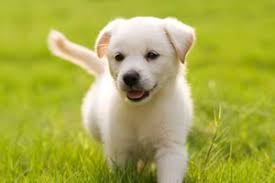
\includegraphics[width=0.4\textwidth]{perro.jpg}%
		\label{fig:perro}
	}
	\hfill
	\subfloat[Gato]{%
		
\includegraphics[width=0.4\textwidth]{gato.jpg}%
		\label{fig:gato}
	}
	\caption{Imagen de dos mascotas}
	\label{fig:mascotas}
\end{figure}